\section{Tightly Coupled / Scratchpad Memory \weekDoran{3}}
	Scratchpad memory is basically a RAM block in the same order of magnitude as the cache in both size and speed. Contrary to cache memory it is mapped into the processor's memory space.
	
	\begin{compactitem}
	  \item No discrimination between code and data.
	  \item Placement either at run-time or compile time.
	\end{compactitem}
	
	\subsection{Static Partitioning \weekPageDoran{3}{47}}
		Memory is divided in different blocks (partitions). The size of the process and the size of the partition is never equal, this causes \textbf{internal fragments}. This can be reduced by making unequal partition sizes and queues for usage of these fragments. 
	\subsection{Dynamic Partitioning \weekPageDoran{3}{48}}
		Dynamic partitioning creates partition with the exact same size as the processes. This solves the issue of internal fragments, but causes \textbf{external fragments}.
			
		\subsubsection{Placement Algorithms}
			\begin{minipage}[t]{0.6\textwidth}		
				\begin{table}[H]
					\centering
					\begin{tabular}{|p{0.25\linewidth}|p{0.6\linewidth}|}
						\hline
						\textbf{First Fit}
							& Scan memory from top and take first fit. Tends tobe the simplest and produces less fragmentation than \textbf{Next Fit}.\\
						\hline
						\textbf{Next Fit}
							& Scan memory from last allocation and take next best fit.\\
						\hline
						\textbf{Best Fit}
							& Scan entire memory and find best fit out of all possibilities. Causes lots of little fragments.\\
						\hline	
					\end{tabular}
					%\caption{Dynamic Partitioning Placement Algorithms}
				\end{table}
			\end{minipage}
			\begin{minipage}[t]{0.4\textwidth}
				\vspace{0pt}
				
				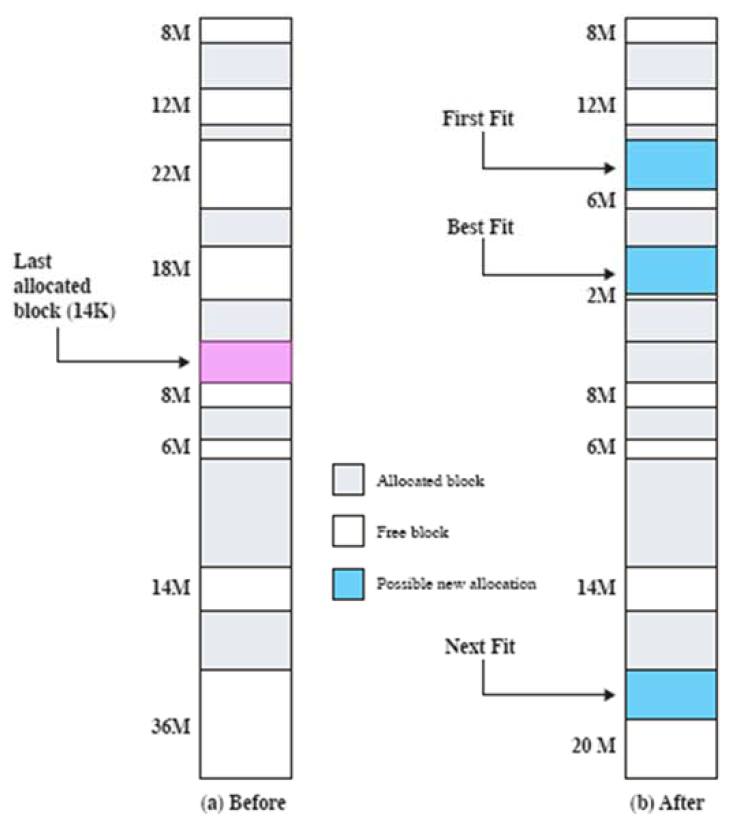
\includegraphics[width=1.1\textwidth]{./pictures/dynamic_partitioning.png}
			\end{minipage}
			
	\subsection{Paging \weekPageDoran{3}{49}}
		Process image is divided into pages of a specific size and divide available memory into frames of equal size. Management is done by a \textbf{page table} where entries are the frame numbers and the reference is the page number. 
		
		\begin{tabular}{p{0.475\textwidth}p{0.475\textwidth}}
			\vspace{0pt}
			
			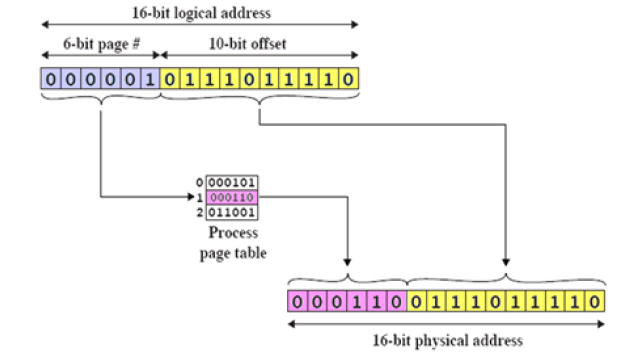
\includegraphics[width=0.45\textwidth]{./pictures/pagingAddressTrans.png}
			& \vspace{0pt}
			
			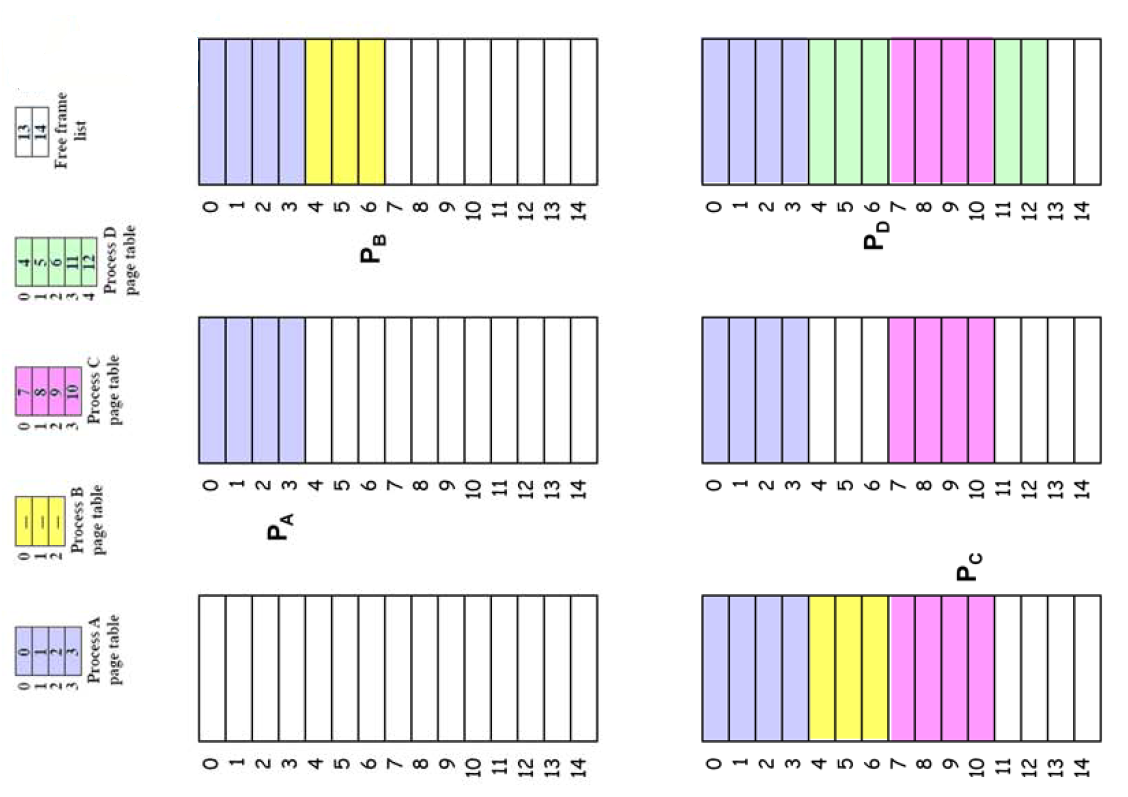
\includegraphics[width=0.45\textwidth, height=10cm]{./pictures/paging.png}
		\end{tabular}	
		